\scanpage{521}
\mspage{266}

qui identifie $\mathcal E_{0,3}$ à un ss-groupe \inserted{\unsure{ouvert}\illegible{1}} d'indice $6$ de $\mathcal E'_{1,1}=\mathcal E_{1,1}/(\pm1)$, et itou pour $\widehat\Pi_{0,3}$ dans $\widehat{\mathcal T}_{1,1}^{\prime+}$. On trouve ainsi un iso\deleted{\illegible{1}}morphisme
\[
(32)\qquad
\widehat\Pi_{0,3}\xrightarrow{\sim}
\begin{gathered}
\operatorname{Ker}(\widehat{\mathcal T}_{1,1}^{\prime+}\longrightarrow\unsure{\mathfrak S}_3)\\
\wr\\
\biggl(\operatorname{Ker}\biggl(
\begin{gathered}\widehat{\mathcal T}_{11}^{+}\\\wr\\\mathrm{Sl}(2,\mathbb Z)^{\wedge}\end{gathered}
\longrightarrow
\begin{gathered}\unsure{\mathfrak S}_3\\\wr\\\mathrm{Sl}(2,\mathbb F_2)\end{gathered}
\biggr)\biggr)/\pm1
\end{gathered}
\]
compatible avec les actions extérieures de $\Gamma$. On peut dire aussi qu'on a une structure d'extension
\[
(33)\qquad
\diagram{\begin{tikzcd}[ampersand replacement=\&,column sep=small]
1\arrow[r,dash] \& \widehat\Pi_{0,3}\arrow[r] \& \widehat{\mathcal T}_{1,1}^{\prime+}\arrow[r]\arrow[d,phantom,"\wr" description] \& \unsure{\mathfrak S}_3\arrow[r]\arrow[d,phantom,"\wr" description] \& 1\\
\&\&\mathrm{Sl}(2,\mathbb Z)^{\wedge}/\pm1\arrow[r]\&\mathrm{Sl}(2,\mathbb Z_{/2})\&
\end{tikzcd}}
\]
compatible avec les actions de $\Gamma$ ($\Gamma$ opérant trivialement sur $\unsure{\mathfrak S}_3$).

Je finis par m'apercevoir que ce qu'on obtient ici est loin de 22 --- cet hom. (22) n'a rien d'injectif, par contre il est surjectif --- et ses valeurs sont \unsure{non} dans $\mathrm{Sl}(2,\mathbb Z)/\pm1$, mais dans $\mathrm{Sl}(2,\mathbb Z)$ lui-$\overline{\mathrm m}$! Il faudra donc que je \unsure{revienne} encore sur une façon de donner
\scanpage{522}
un sens arithmético-géométrique remarquable à (22), et son \unsure{extension} aux groupes profinis correspondants. Pour le moment, je m'en tiens à exploiter un peu (33). Tout d'abord je note que les arguments faits dans le cadre schématique, marchent aussi dans le cas transcendant, analytique complexe, et fournissent alors
\[
(34)\qquad
\Pi_{0,3}\xrightarrow{\sim}\operatorname{Ker}\biggl(
\begin{gathered}\mathcal T_{11}^{\prime+}\\\Vert\\\mathrm{Sl}(2,\mathbb Z/2\mathbb Z)/\pm1\end{gathered}
\longrightarrow
\begin{gathered}\unsure{\mathfrak S}_3\\\Vert\\\mathrm{Sl}(2,\mathbb Z/2\mathbb Z)\end{gathered}
\biggr)
\]
compatible avec (32), ou encore une suite exacte
\[
(35)\qquad
\diagram{\begin{tikzcd}[ampersand replacement=\&,column sep=small]
1\arrow[r,dash]\&\Pi_{0,3}\arrow[r]\&\mathcal T_{11}^{\prime+}\arrow[r]\arrow[d,phantom,"\wr" description]\&\unsure{\mathfrak S}_3\arrow[r]\arrow[d,phantom,"\wr" description]\&1\\
\&\&\mathrm{Sl}(2,\mathbb Z)/\pm1\&\mathrm{Sl}(2,\mathbb Z/2\mathbb Z)\&
\end{tikzcd}}\unsure{,)|.,}
\]

\deleted{\unsure{qui}} On aimerait interpréter (35) et (33) comme correspondant \unsure{aux} suites exactes analogues liées au diagramme (\unsure{9}), reliant $\Pi_{0,3}$ et $\Pi'_{0,3}$ --- en identifiant $\Pi'_{0,3}$ à $\mathcal T_{11}^{\prime+}$, $\widehat\Pi'_{0,3}$ à $\widehat{\mathcal T}_{11}^{\prime+}$. J'y reviendrai \unsure{tantôt}.

\uline{Rem.} On peut se demander si l'hom
\[
\widehat\Pi_{0,3}\longrightarrow\mathrm{Sl}(2,\mathbb Z)^{\wedge}/\pm1\simeq\widehat{\mathcal T}_{11}^{+}/(\pm1)
\]
se remonte (de façon plus ou moins naturelle)
\scanpage{523}
\mspage{267}
en un hom
\[
\widehat\Pi_{0,3}\longrightarrow\mathrm{Sl}(2,\mathbb Z)^{\wedge}\simeq\deleted{\unsure{\mathrm{Sl}}}\widehat{\mathcal T}_{1,1}^{+}
\]
et itou pour les groupes discrets
\[
\Pi_{0,3}\longrightarrow\mathrm{Sl}(2,\mathbb Z)\simeq\mathcal T_{11}^{+}.
\]

\margin{Oui, on peut remonter, et c'est plus ou moins trivial... cf plus bas...}

Bien sûr, comme $\Pi_{0,3}$ et $\widehat\Pi_{03}$ sont libres (avec deux \unsure{gén}) on peut tjrs remonter --- \deleted{\unsure{l'indétermination à}}\inserted{d'exactement} \uline{quatre} façons, d'ailleurs. (qui nécessairement, dans le cadre profini, \unsure{respectent} les réseaux discrets). Mais peut-on le faire en \unsure{respectant} les op. de $\Gamma$? Il suffirait pour cela qu'on puisse remonter $U_{0,3}\longrightarrow M'_{1,1}\deleted{[2]}$ en $U_{0,3}\longrightarrow M_{11}^{\unsure{t|\ell}}$ (\uline{NB} $M_{11}$ est une \deleted{\illegible{1}} $\mathbb Z/2$-gerbe au dessus de $M'_{11}$) --- et je suspecte, \deleted{que}
\margin{pas tout à fait cf \unsure{pg} suivante pour une formulation plus \unsure{raisonnable}...}
d'après le \unsure{yoga} ``anabélien'' que j'essaye de développer, que l'inverse doit être vrai --- que tt relèvement de $\widehat\Pi_{03}\longrightarrow\widehat{\mathcal T}_{11}^{\prime+}\deleted{\unsure{\Pi}}$ \unsure{commutant} aux op. de $\Gamma$ est défini par un tel relèvement $U_{0,3}\longrightarrow M_{1,1}$. Or l'existence \inserted{d'un tel relèvement $U_{0,3}\longrightarrow M_{1,1}$} signifierait \inserted{\unsure{exactement}} l'existence d'une famille de courbes elliptiques sur $U_{0,3}$, avec
\scanpage{524}
rigidification de Jacobi d'échelon $2$, qui \unsure{corresponde} à l'invariant tautologique $\lambda$. Je doute qu'il en existe une, comme je doute que le relèvement en termes de groupes profinis à op. puisse se faire.

À vrai dire, comme \inserted{$\widehat{\mathcal T}_{11}^{+}=$}$\mathrm{Sl}(2,\mathbb Z)^{\wedge}$ n'a plus de centre trivial, il n'est plus \deleted{licite} \inserted{raisonnable à vrai dire} de \unsure{vouloir} ``\unsure{tout exprimer}'' \unsure{par} les \unsure{op.} ext. de $\Gamma$ sur $\widehat{\mathcal T}_{11}^{+}$, il faut plutôt revenir à l'extension $\mathcal E_{11}=\mathcal E_{M_{1,1}}$ de $\Gamma$ par $\widehat{\mathcal T}_{1,1}^{+}$, et la question est si l'homomorphisme
\[
\mathcal E_{0,3}\longrightarrow\mathcal E'_{1,1}=\mathcal E_{1,1}/\pm1
\]
se remonte en
\[
\mathcal E_{0,3}\xrightarrow{?}\mathcal E_{11},
\]
\deleted{\unsure{choisissant un}}\inserted{ce qui est plus} fort que de trouver un relèvement $\widehat{\Pi}_{0,3}\longrightarrow\mathcal T_{11}^{+}$ compatible avec les \unsure{op.} ext. de $\Gamma$. Pour \unsure{apprécier} cette différence, je note que $\Gamma$ opère sur l'ens\inserted{ $E$} des quatre relèvements \unsure{de} $\widehat{\Pi}_{0,3}\longrightarrow\widehat{\mathcal T}_{1,1}^{+}$, (\unsure{interprétés} comme hom. extérieurs), et la
\scanpage{525}
\mspage{268}
question posée sous la forme faible est s'il existe un élément de $E$ invariant par $\Gamma$. S'il n'en existait pas, il y aurait en tous cas un sous-groupe ouvert de $\Gamma$, d'indice \deleted{divisant}\inserted{$2$ ou $4$} \deleted{\illegible{1} $4$, tel que} \inserted{\deleted{$4!=24$,} qui} laisserait invariant un élément --- donc quitte à passer à l'extension \deleted{\illegible{1}} finie correspondante de $\mathbb Q$, on trouve le relèvement --- et quitte à passer à une extension un peu plus grande, les \uline{quatre} relèvements possibles commutent à l'action ext. de $\Gamma$. Par contre, rien ne prouve que l'on puisse trouver un \inserted{``germe de} relèvement'' \deleted{\unsure{$\mathcal E_{0,3}\longrightarrow\mathcal E_{11}$}} de $\mathcal E_{0,3}\longrightarrow\mathcal E'_{1,1}$ en \unsure{$\mathcal E_{0,3}^{G}\longrightarrow\mathcal E_{1,1}^{G}$} (\unsure{germes} pris p.r. aux sous-groupes \inserted{\unsure{ouverts|ouvert}} de $\mathcal E_{0,3}$ \deleted{\illegible{1}} contenant $\widehat\Pi_{0,3}$, ou $\overline{\mathrm m}$ de tt les sous-groupes ouverts) L'obstruction à \deleted{\illegible{3}}\inserted{\unsure{remonter sur}} $\mathcal E_{0,3}$ \deleted{\illegible{3}}\inserted{lui $\overline{\mathrm m}$}, i.e. à \uline{\unsure{scinder}} une certaine extension de $\mathcal E_{0,3}$ par \deleted{\unsure{$\mathbb Z$}} $\pm1$), est
\figure{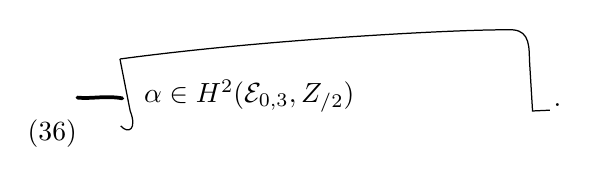
\begin{tikzpicture}[x=1cm,y=1cm,baseline=(formule.base)]
\node[anchor=west,inner sep=0pt] (formule) at (1.02,0)
  {$\alpha\in H^2(\mathcal E_{0,3},\mathbb Z_{/2})$};
\node[anchor=east,inner sep=0pt] at (0.18,-0.48) {$(36)$};
\draw[line width=0.45pt]
  (0.72,0.47) .. controls (2.65,0.73) and (5.13,0.85) .. (5.64,0.84)
  .. controls (5.89,0.86) and (5.92,0.70) .. (5.92,0.47)
  -- (5.96,-0.19) -- (6.18,-0.18);
\draw[line width=0.45pt]
  (0.72,0.47) -- (0.85,-0.19)
  .. controls (0.94,-0.42) and (0.83,-0.49) .. (0.73,-0.38);
\draw[line width=1.35pt,line cap=round]
  (0.18,-0.02) .. controls (0.35,-0.04) and (0.55,0.01) .. (0.75,-0.03);
\node[anchor=west,inner sep=0pt] at (6.22,-0.12) {.};
\end{tikzpicture}}
--- et rien ne dit que cette classe de cohomologie puisse s'effacer, en passant à un ss-groupe ouvert de $\mathcal E_{0,3}$.
\figure{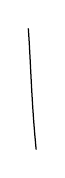
\begin{tikzpicture}[x=1cm,y=1cm]
\draw[line width=0.45pt]
  (0,1.05) .. controls (0.03,0.64) and (0.04,0.11) .. (0.10,-0.49);
\end{tikzpicture}}

\scanpage{526}

Mais en termes géométriques, \deleted{\unsure{bientôt}} les courbes elliptiques relatives \unsure{cherchées} sur \unsure{$U_{0,2}$|$U_{0,3}$} forment \unsure{\deleted{les}|les} sections d'un champ sur $(U_{0,3})_{\mathrm{et}}$, qui est une \deleted{\unsure{$\{\pm1\}$}}\inserted{$\mathbb Z_{/2}$}-gerbe --- l'obstruction se trouve donc dans un groupe de Brauer
\[
\beta\in H^2(U_{0,3},\mathbb Z_{/2}), \tag{37}
\]
or comme $U=U_{0,3}$ est une courbe alg. \deleted{\illegible{1}} affine sur un corps (il \unsure{suffirait} qu'elle ne soit de type $0,0$) \unsure{il s'ensuit} que l'hom canonique (à coefficients de torsion quelconques)
\[
H^*(\mathcal E_U,-)\longrightarrow H^*(U,-)
\]
est un iso. D'ailleurs, il \unsure{doit} être $\pm$ trivial que $\beta$ est l'image de $\alpha$ --- ce qui confirme l'\unsure{intuition|intention} que \deleted{\unsure{le}} si le relèvement est possible au niveau des groupes fondamentaux profinis (\unsure{arithmético-géométriques|arithmético-géométrique}) il l'est aussi au niveau des \unsure{multiplicités} modulaires elles-$\overline{\mathrm m}$, donc qu'on a une existence d'une courbe elliptique relative sur $U_{0,3}$ qui\ldots

\scanpage{527}
\mspage{269}

Il est \unsure{vrai} qu'il est bien \unsure{connu} qu'une classe de cohomologie (37) à coeff de torsion s'efface, en \unsure{passant} à une extension finie du \deleted{\unsure{$\mathbb Q$}} corps de base ($\mathbb Q$ en l'occurrence). En fait, on a une suite spectrale
\[
(38)\qquad H^*(U_{0,3},\mathbb Z_{/2})
\Longleftarrow E_2^{pq}
=H^p(\deleted{\unsure{\overline U_{0,3}}}\unsure{\mathbb Q},H^q(\overline U_{0,3},\mathbb Z_{/2}\unsure{)|))}
\]
et ici $H^q(\overline U_{0,3})=0$ pour $q\geq 2$, donc on trouve une suite exacte
\[
\deleted{\unsure{H^1(\mathbb Q)}\longrightarrow
\unsure{H^1(U_{0,3},\mathbb Z_{/2})}\longrightarrow
\unsure{H^1(\overline U_{0,3},-)}}
\]
\diagram{\begin{tikzcd}[ampersand replacement=\&,column sep=small]
\cdots \& E_2^{0,1} \arrow[r] \arrow[d,equal]
\& E_2^{2,0} \arrow[r] \arrow[d,equal]
\& \deleted{\unsure{E}}H^2(U_{0,3}) \arrow[r]
\& E_2^{1,1} \arrow[r] \arrow[d,equal]
\& E_2^{3,0} \arrow[d,equal] \& \cdots \\
\& H^0(\mathbb Q,H^1(\overline U)
\& H^2(\mathbb Q,\mathbb Z_{/2})
\&
\& H^1(\mathbb Q,\underset{\substack{\wr\\\mathbb F_2^2}}{H^1(\overline U)})
\& H^3(\mathbb Q,\unsure{\mathbb Z_{/2}|\mathbb F_2}) \&
\end{tikzcd}}

Je me \unsure{rends} compte enfin que l'existence d'un \deleted{\illegible{1}} relèvement, -- i.e. de la courbe elliptique hypothétique sur $U_{0,3}$ -- est tout à fait triviale, il suffit de \unsure{la|le} définir par l'équation
\[
y=\sqrt{\unsure{x|\dot x}(x-1)(x-\lambda)}
\]
i.e.
\[
y^2-x(x-1)(x-\lambda)=F(x,y;\lambda]=0
\]
ce qui définit une courbe plane affine,
\scanpage{528}
\unsure{on passe|ou passer} en coordonnées projectives
\[
F(x,y,z;\lambda)=y^2z-x^3+(1+\lambda)x^2z-\lambda xz^2=0
\]
\deleted{\unsure{pour|puis}} Je ne vais pas approfondir la question ici\unsure{.} \unsure{dans} quelle mesure ce choix est ``naturel''.

\deleted{\unsure{Une fois}} \inserted{\unsure{Il}} donne en tous cas un \unsure{homomorphis-}\deleted{\unsure{me extérieur}} \unsure{tout} ce qu'il y a de précis
\[
(39)\qquad M_{0,4}^{!}=U_{0,3}\longrightarrow M_{1,1}
\]
d'où un \unsure{hom.|hom} d'extensions
\diagram{\begin{tikzcd}[ampersand replacement=\&,column sep=small,row sep=small]
\& \& \widehat{\mathcal T}_{0,4}^{!+} \arrow[d,phantom,"\wr" description]
\& \unsure{N_{0,4}^{!}|\mathcal N_{0,4}^{!}} \arrow[d,phantom,"\wr" description] \& \& \\
(40) \& 1 \arrow[r]
\& \widehat\Pi_{0,3} \arrow[r] \arrow[d]
\& \mathcal E_{0,3} \arrow[r] \arrow[d]
\& \Gamma \arrow[r] \arrow[d,equal] \& 1 \\
\& 1 \arrow[r]
\& \widehat{\mathcal T}_{11}^{+} \arrow[r] \arrow[d,phantom,"\wr" description]
\& \mathcal E_{11} \arrow[r] \arrow[d,equal]
\& \Gamma \arrow[r] \& 1 \\
\& \& \unsure{\mathrm{Sl}}(2,\mathbb Z)^{\wedge}
\& \unsure{N_{1,1}|\mathcal N_{1,1}}\deleted{\unsure{\simeq\mathrm{Sl}(2,\mathbb Z)^{\wedge}}} \& \&
\end{tikzcd}}
défini mod \unsure{autom.|autom} \unsure{intérieure} par \deleted{et} un élément de $\widehat{\mathcal T}_{11}^{+}\simeq\unsure{\mathrm{Sl}}(2,\mathbb Z)^{\wedge}$, et au niveau des groupes \unsure{discrets|discret}
\[
\deleted{(41)}\qquad \Pi_{0,3}\longrightarrow\mathcal T_{1,1}^{+}
\]
\deleted{\unsure{mais} il n'est plus tellement}
\inserted{et même}
\[
(42)\qquad \Pi_{0,3}\hookrightarrow
\overbrace{\operatorname{Ker}\left(
\underset{\substack{\Vert\\\unsure{\mathrm{Sl}}(2,\mathbb Z)}}{\mathcal T_{1,1}^{+}}
\longrightarrow
\underset{\substack{\Vert\\\unsure{\mathrm{Sl}}(2,\mathbb Z_{/2})}}{\unsure{\mathfrak S_3}}
\right)}^{\unsure{\Gamma_2}}
\]
(et itou pour les groupes profinis). Ici $\Pi_{0,3}$ est tel que le sous-groupe de congruence du \unsure{deuxième} \unsure{mb|niv.} \deleted{\unsure{$\Gamma$}} soit $\unsure{\Gamma_2}$, \unsure{soit|est} produit direct de \unsure{ce|le} \unsure{sous-groupe|sous-groupes} $\Pi_{0,3}$ et de
\scanpage{529}
\mspage{270}
son centre $\pm1$. (Mais en fait, il y a \unsure{exactement} quatre sous-groupes de $\Gamma_2$ qui \unsure{réalisent} cette décomposition. Pour ne pas faire \unsure{de|des} jaloux, on pourrait regarder l'intersection des quatre, qui est un sous-groupe $\Gamma_2$ d'indice un diviseur de $2^4=16$ c'est l'intersection des noyaux \unsure{de|des} quatre homomorphismes $\Gamma_2\longrightarrow\deleted{\mathbb Z_{/2}}\ \unsure{\mathrm{Centre}}(\Gamma_2)=\{\pm1\}$,
\margin{\uline{NB} \unsure{Ça} doit être le noyau de $\mathrm{Sl}(2,\mathbb Z)^{\unsure{\wedge|*}}\longrightarrow\mathrm{Sl}(2,\mathbb Z/4\mathbb Z)$}
En tant que sous-groupe de $\Pi_{0,3}$, il est d'indice un diviseur de $8$ -- Ça m'étonnerait pas que ce soit juste le groupe des commutateurs de $\Pi_{0,3}$,) qui est d'indice $4$ -- il y a là toute une \unsure{situation} à élucider\ldots\,.
\margin{c'est vrai et c'est \unsure{$\simeq$|$\overline{\mathrm m}$} trivial\ldots}
\margin{Il n'est pas clair \deleted{si $\Pi_{0,3}$} est invariant en \unsure{tant} que ss-groupe de \deleted{\unsure{$\mathfrak S$}} $\mathcal T_{1,1}^{+}\simeq\mathrm{Sl}(2,\mathbb Z)$, i.e. stable par l'action ext. de $\unsure{\mathfrak S}_3$ sur $\mathrm{Sl}(2,\mathbb Z)$ -- je présume que oui, puisque $\unsure{\mathfrak S}_3$ opère aussi extérieurement sur $\Pi_{0,3}$ a priori\ldots\ $\mathcal T_{11}^{+}/\Pi_{0,3}$ serait une extension centrale \unsure{intéressante} de $\unsure{\mathfrak S}_3$ par $\{\pm1\}$\ldots}

Bien entendu, il faudrait aussi expliciter l'homomorphisme (42) (défini \unsure{mod} \unsure{autom.} intérieurs) par ses valeurs sur les générateurs $\unsure{l_0,l_1,l_2}$ -- j'y reviendrai peut-être tantôt.

\scanpage{530}

\uline{Théorème} L'action extérieure naturelle de $\Gamma_Q$ sur $\widehat{\mathcal T}_{1,1}^{+}$, et même sur $\widehat{\mathcal T}_{1,1}^{+\prime}=\widehat{\mathcal T}_{1,1}/(\pm1)$, est fidèle.
\figure{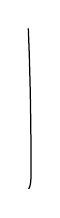
\begin{tikzpicture}[x=1cm,y=1cm]
\draw[line width=0.45pt]
  (0,1.05) .. controls (0.025,0.44) and (0.035,-0.19) .. (0.035,-0.78)
  .. controls (0.035,-0.91) and (0.025,-0.96) .. (0.005,-0.99);
\end{tikzpicture}}

On utilise le fait qu'on a un hom. ext. injectif
\[
\widehat{\Pi}_{0,3}\hookrightarrow\widehat{\mathcal T}_{1,1}^{\prime+}
\]
compatible avec l'action de $\Gamma$, en procédant comme pour la proposition du début (où $\widehat{\Pi}_{0,3}'$ jouait le rôle de $\widehat{\mathcal T}_{1,1}^{\prime+}$).

\uline{Corollaire} Les homomorphismes canoniques (surjectifs)
\[
\tag{43}
\Gamma_Q\longrightarrow\Gamma_{1,\nu}\qquad(\nu\geq1)
\]
sont injectifs, donc des isomorphismes.

Il suffit de le prouver pour $\Gamma_Q\longrightarrow\Gamma_{1,1}$ (puisque $\Gamma_{1,1}$ est un quotient de $\Gamma_{1,\nu}$, $\nu\geq1\ldots$), or on a un hom \unsure{\deleted{\illegible{1}}} $\Gamma_{1,1}\longrightarrow\mathrm{Aut\ ext}\,\widehat{\mathcal T}_{1,1}^{+}$ et on peut considérer le \unsure{composé}
